\chapter{Experimente}
\label{cha:experimente}

\section{Alternative Kalibrierung}
\label{sec:alternativekalibrierung}

\begin{figure}[H]
	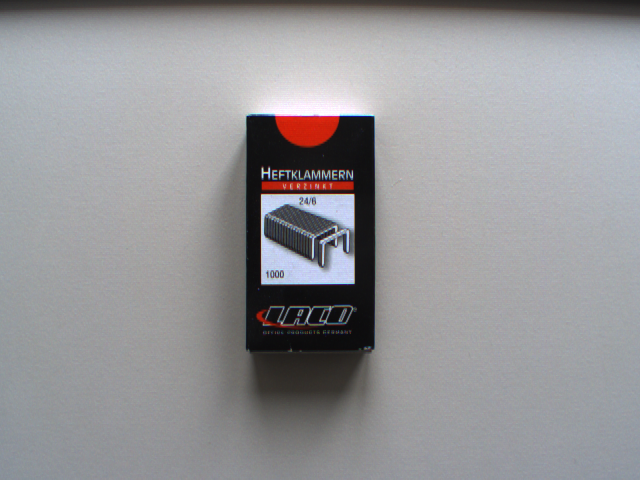
\includegraphics[scale=1.0]{bilder/experimentcalib}
	\caption[Kalibrierung Alternative]{Kalibrierung Alternative}
\end{figure}

\section{Tiefeninformationen}
\label{sec:expiefeninformationen2}

$Z=\frac{f*B}{x-x'}$
$f=1192$ und $B=33.5$(cm)

\begin{figure}[H]
	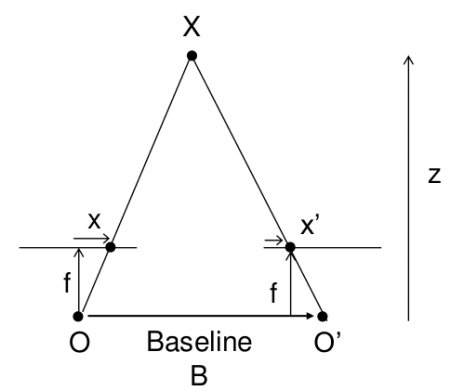
\includegraphics[scale=1.0]{bilder/tiefenberechnung}
	\caption[Tiefenberechnung]{Tiefenberechnung}
\end{figure}

\begin{figure}[!htb]
	\minipage{0.32\textwidth}
	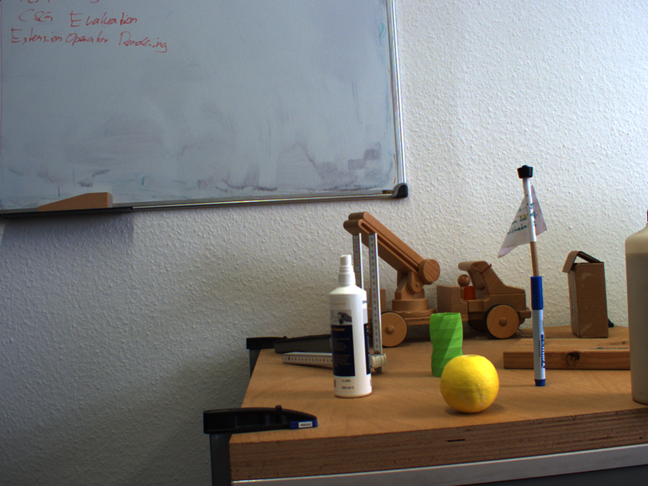
\includegraphics[width=\linewidth]{bilder/depth_left}
	\caption{Tiefe links}\label{fig:awesome_image1}
	\endminipage\hfill
	\minipage{0.32\textwidth}
	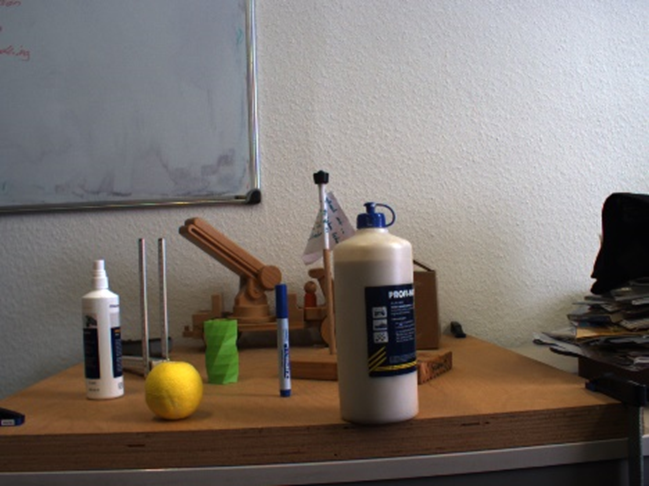
\includegraphics[width=\linewidth]{bilder/depth_right}
	\caption{Tiefe rechts}\label{fig:awesome_image2}
	\endminipage\hfill
	\minipage{0.32\textwidth}%
	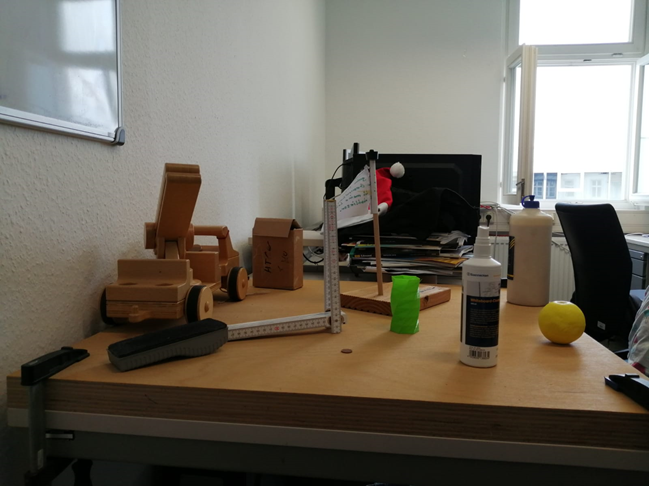
\includegraphics[width=\linewidth]{bilder/depth_side}
	\caption{Tiefe seitlich}\label{fig:awesome_image3}
	\endminipage
\end{figure}

\begin{figure}[!htb]
	\minipage{0.48\textwidth}
	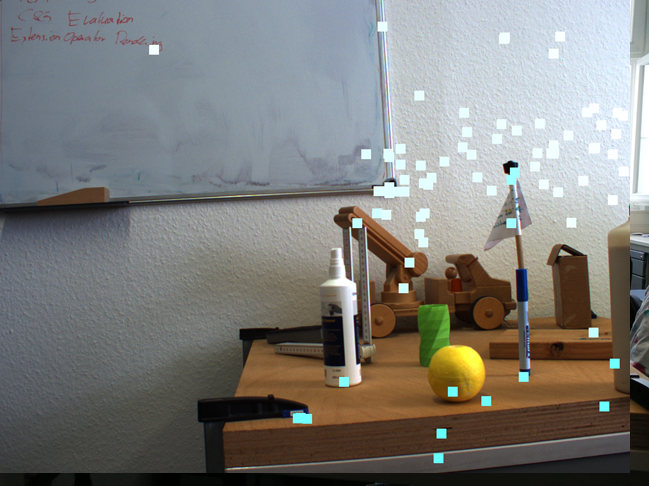
\includegraphics[width=\linewidth]{bilder/depth_result}
	\caption{Tiefeninformation Punkte}\label{fig:awesome_image1}
	\endminipage\hfill
	\minipage{0.48\textwidth}
	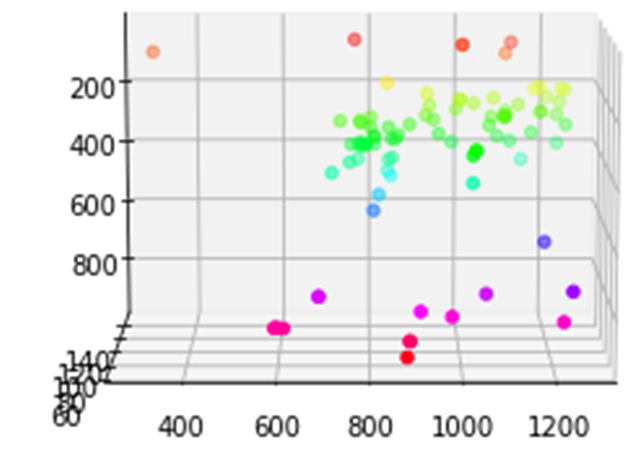
\includegraphics[width=\linewidth]{bilder/depth_coord}
	\caption{Tiefeninformation 3D-Plot}\label{fig:awesome_image2}
	\endminipage\hfill
\end{figure}